% Chapter 5: Temporal Evolution and Dynamic Profiles

\section{Temporal Trajectories of Structural Metrics}

Chapter 4 described the full-period morphology of fields and subfields. This chapter asks whether those profiles stay stable or change over time. I use five fixed windows: 2000--2004, 2005--2009, 2010--2014, 2015--2019, and 2020--2024. Within each window, I recompute the same eight structural metrics used in the static profile. This keeps the temporal analysis directly comparable with the static one.

Each subfield-window is treated as a separate document cloud. The windowed plots use robust-scaled values computed across all completed subfield-window observations. The temporal matrix is almost complete: 1,204 of 1,205 expected subfield-window rows were computed. Computational Mathematics in 2000--2004 is excluded only when a first--last comparison requires a complete trajectory.

The broad movement is toward closer local packing. Across all subfields, mean median centroid distance declines from 0.0858 in 2000--2004 to 0.0750 in 2020--2024. Mean median kNN distance declines from 0.0923 to 0.0756, and PCA \(D_{80}\) falls from 81.3 to 71.1. At the same time, kNN distance variability rises. This is not a simple contraction. The retained document clouds become closer locally on average, but the local spacing becomes less even.

These metrics describe different parts of the same movement. A lower centroid median means that papers are closer, on average, to the window centroid. A lower median kNN distance means that nearby papers are closer to each other. A lower PCA \(D_{80}\) means that fewer principal directions are needed to describe most of the variation. When kNN distance variability rises at the same time, the interpretation becomes more nuanced: some local neighborhoods tighten more than others. Figure~\ref{fig:domain_temporal_trajectories} should therefore be read as a set of related changes, not as eight independent trends.

\begin{figure}[H]
\centering
\caption[Domain-level temporal trajectories]{Domain-level temporal trajectories across five-year windows. Values are mean standardized subfield-window structural metrics within each domain.}
\label{fig:domain_temporal_trajectories}
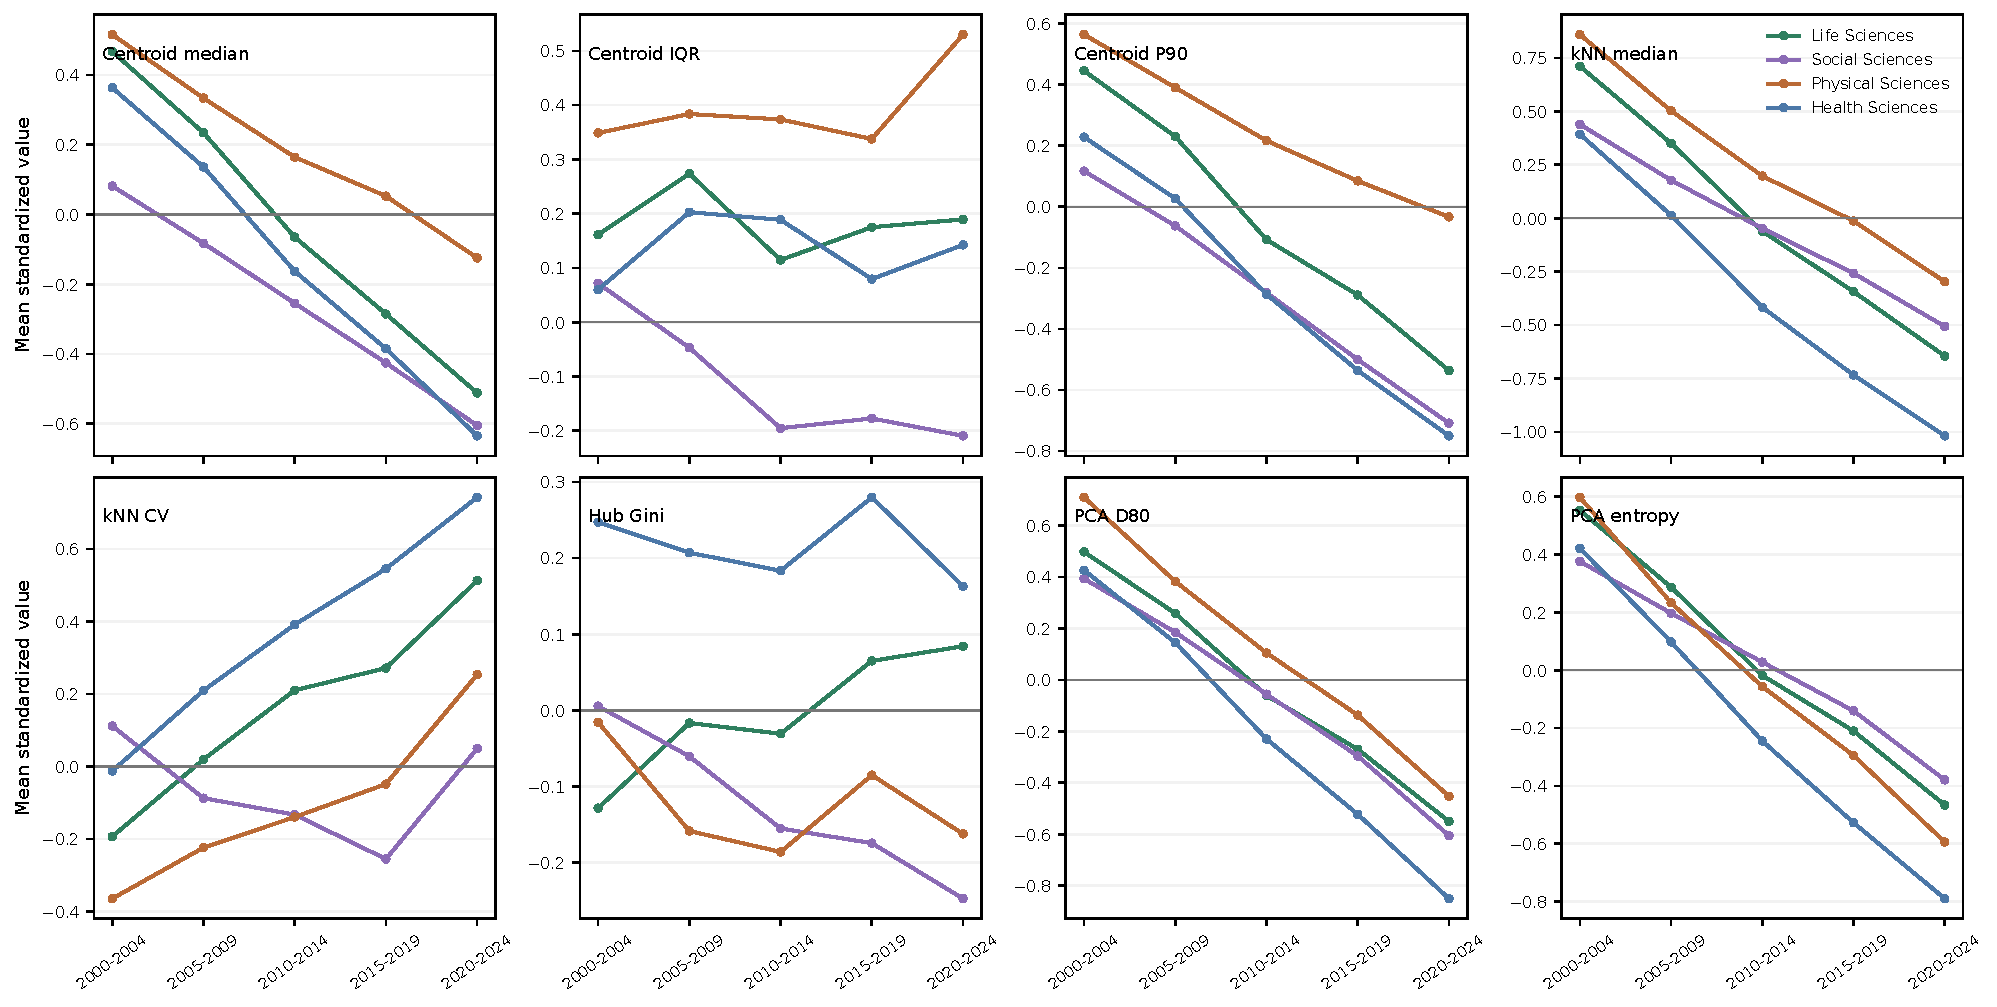
\includegraphics[width=\textwidth]{figures/fig_07_domain_temporal_trajectories.pdf}
\end{figure}

The domain trajectories give a first orientation. Physical Sciences remain the most dispersed domain for most of the period and keep the highest average spectral dimensionality. Health Sciences move furthest downward in local distance and PCA \(D_{80}\). They finish with the tightest local neighborhoods and the lowest average dimensionality. Life Sciences follow the same direction, with a clearer rise in kNN distance variability. Social Sciences are less extreme in the domain averages. As in the static chapter, this makes the field and subfield levels necessary.

\section{Fields and Subfields in Motion}

Field-level first--last deltas show where the average trajectory is strongest. The heatmap compares standardized field profiles in 2020--2024 with their profiles in 2000--2004. Negative values mean that the metric is lower at the end of the period, and positive values mean that it is higher. These changes should be read as changes in shape, not as improvement or decline.

Median centroid distance declines most clearly in Energy, Medicine, Dentistry, Chemical Engineering, and Pharmacology, Toxicology and Pharmaceutics. Median kNN distance declines most clearly in Dentistry, Energy, Medicine, Chemistry, and Immunology and Microbiology. Hubness does not follow the same direction. Energy and Immunology and Microbiology move upward in hub concentration, while Computer Science, Engineering, Psychology, and Health Professions move downward.

\begin{figure}[H]
\centering
\caption[Field-level temporal change heatmap]{Field-level temporal change from 2000--2004 to 2020--2024. Cells are final-minus-initial standardized structural values.}
\label{fig:field_temporal_delta_heatmap}
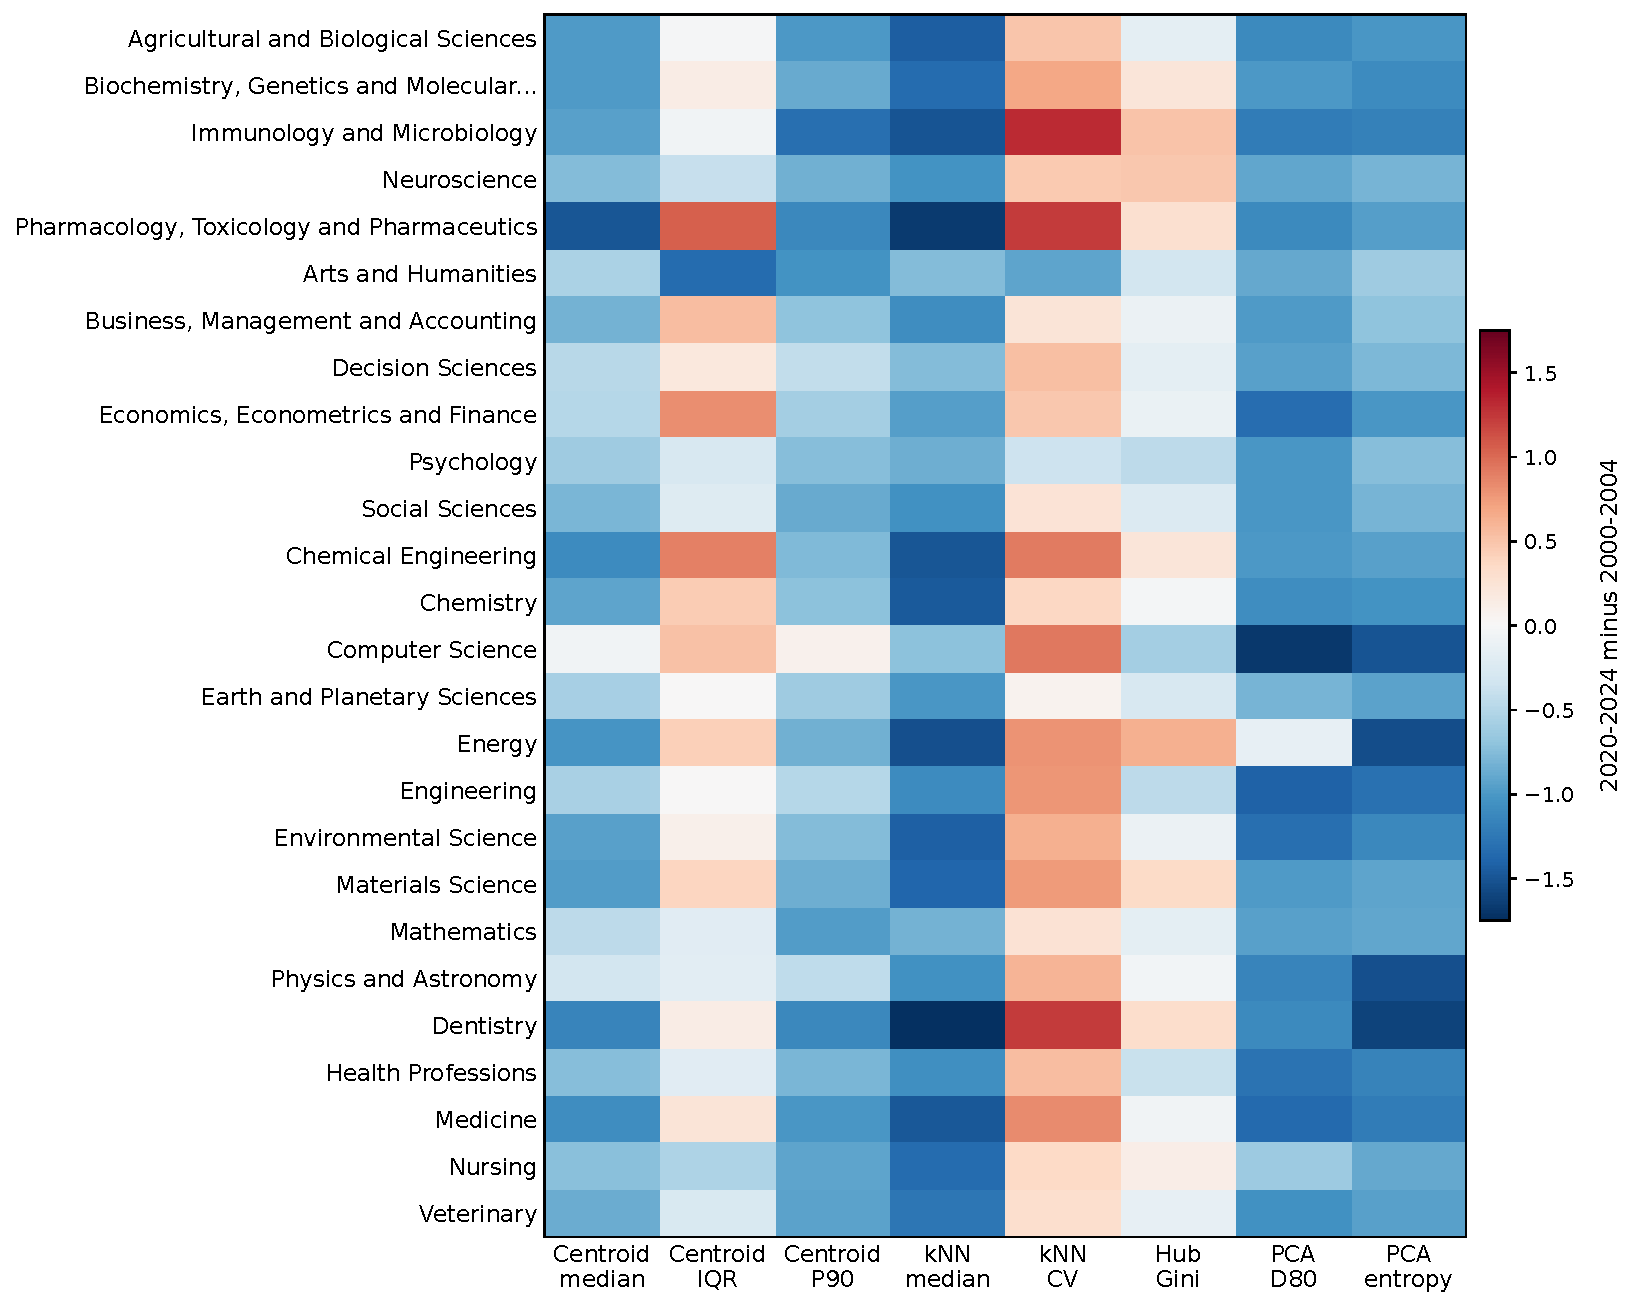
\includegraphics[width=\textwidth,height=0.80\textheight,keepaspectratio]{figures/fig_07_field_temporal_delta_heatmap.pdf}
\end{figure}

The field changes therefore do not describe one universal temporal direction. Some fields become more compact around their centroid or in their local neighborhoods. Other fields change mainly through hubness or spectral structure. This is why the temporal profile keeps the same eight metrics instead of reducing change to one expansion or contraction measure.

The strongest first--last profile changes are concentrated in a small set of subfields. Philosophy has the largest windowed structural displacement, followed by General Dentistry, Molecular Medicine, General Psychology, Immunology and Allergy, Infectious Diseases, Renewable Energy, Sustainability and the Environment, Pharmacy, Instrumentation, and Virology. The ranking measures Euclidean distance between initial and final standardized profiles across the eight windowed structural metrics.

\begin{figure}[H]
\centering
\caption[Most dynamic subfields]{Most dynamic subfields across windowed structural metrics. The ranking measures total first--last profile displacement.}
\label{fig:most_dynamic_subfields}
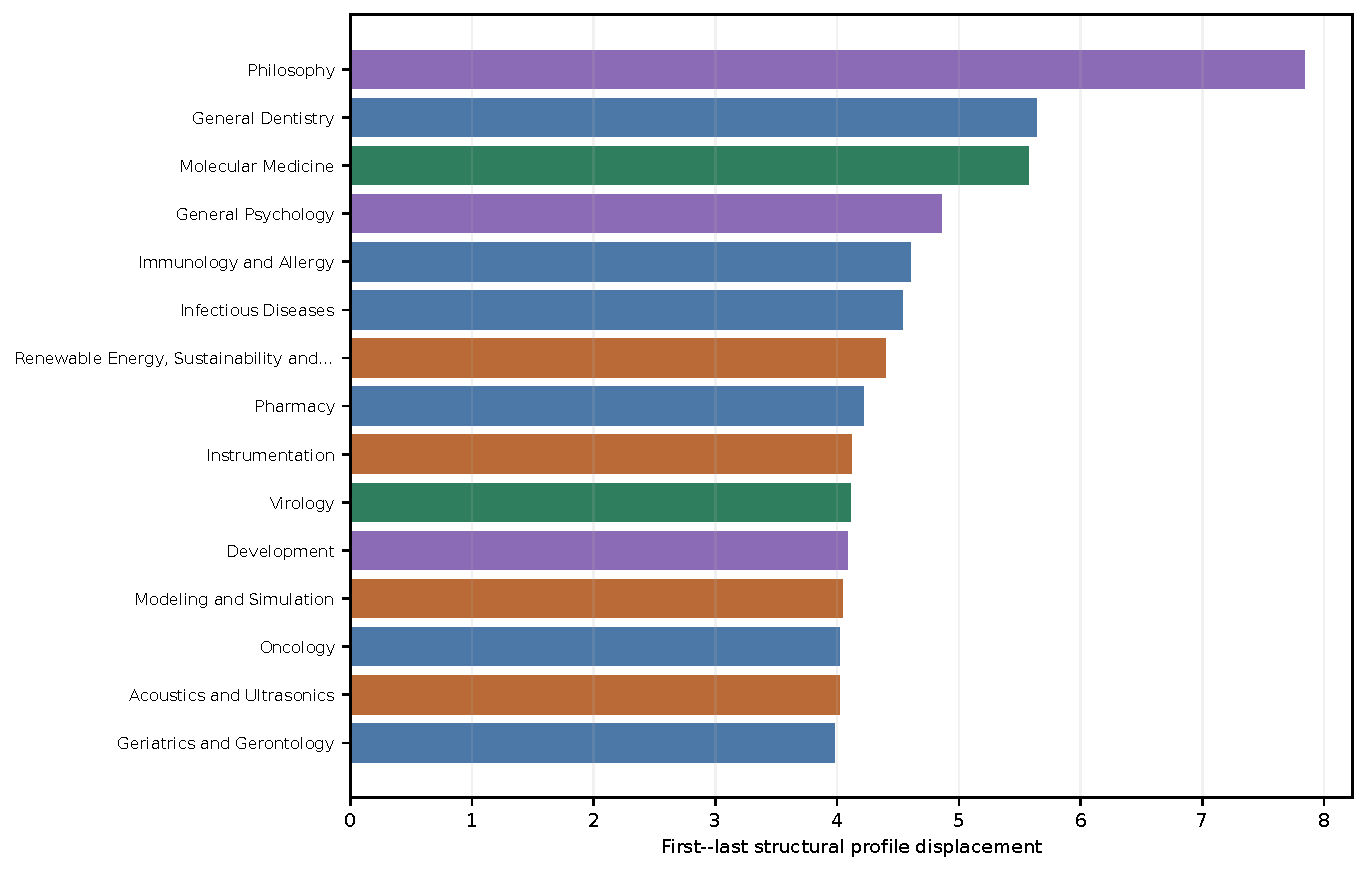
\includegraphics[width=0.93\textwidth]{figures/fig_07_most_dynamic_subfields.pdf}
\end{figure}

The drivers behind these cases are mixed. Philosophy is dominated by a sharp decrease in centroid-distance IQR, while Molecular Medicine moves in the opposite direction on the same metric. General Dentistry is driven by a decline in PCA spectral entropy. General Psychology changes mainly through reduced kNN distance variability. Immunology and Allergy and Virology change through increases in that same metric. The important point is that large temporal movement can come from different structural families.

\section{Net Semantic Displacement}

The eight-metric structural profile describes shape. A separate question is whether the semantic center of a subfield moves across the period. I measure this complementary quantity with early--late centroid drift, the cosine distance between each subfield's 2000--2004 and 2020--2024 centroids. Across analysis subfields, the median drift is 0.0045 and the maximum is 0.0384.

Centroid drift uses the same early and late windows as the first--last structural comparison, but it answers a different question. The structural metrics ask how the papers are arranged around one another. Centroid drift asks how far the average location of the subfield moves in the embedding space.

\begin{figure}[H]
\centering
\caption[Net semantic displacement extremes]{Highest and lowest early--late centroid drift by subfield. Left panel: Subfields with the highest drift (most semantically dynamic). Right panel: Subfields with the lowest drift (most stable).}
\label{fig:centroid_drift_extremes}
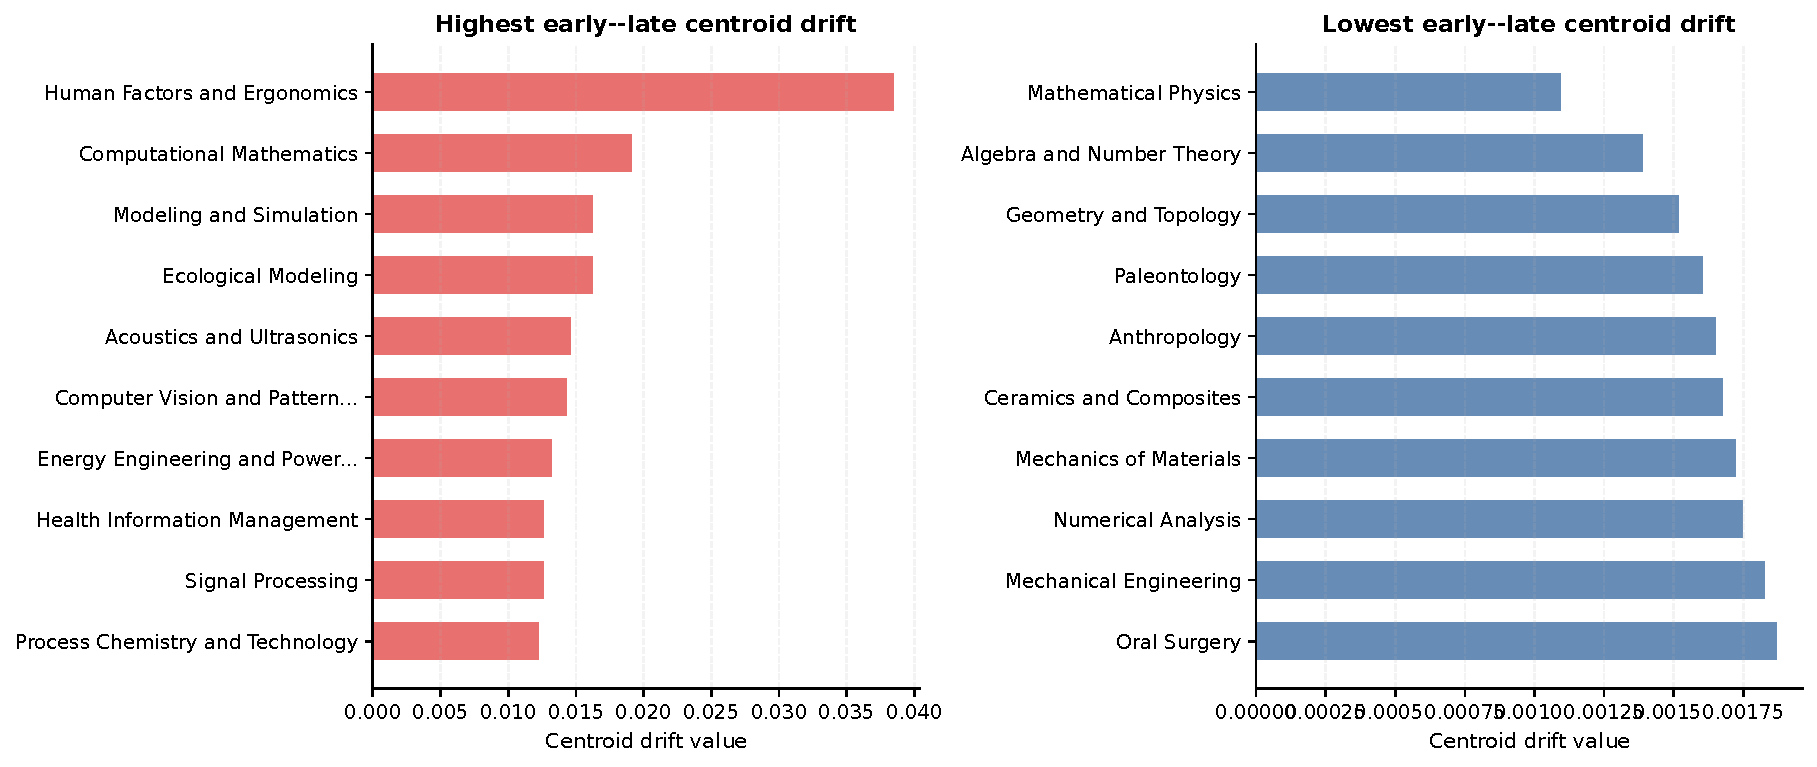
\includegraphics[width=\textwidth]{figures/fig_07_centroid_drift_extremes.pdf}
\end{figure}

The largest net displacement belongs to Human Factors and Ergonomics, followed by Computational Mathematics, Modeling and Simulation, Ecological Modeling, Acoustics and Ultrasonics, and Computer Vision and Pattern Recognition. The most stable centroids include Mathematical Physics, Algebra and Number Theory, Geometry and Topology, Paleontology, and Anthropology.

These cases are not added back into the structural profile. They answer a different diagnostic question after structural shape has already been measured. This separation matters because movement of the center and change in the internal shape are not the same result. A subfield can move in semantic location while keeping a similar profile, or it can reorganize internally while its center remains relatively stable.

\section{Static Shape Versus Temporal Trajectories}
\label{sec:static-dynamic-trajectories}

The useful part of clustering is compression. Static morphology clusters the 241 analysis subfields by eight robust-scaled full-period structural metrics. Dynamic morphology clusters the 240 complete subfields by the slopes of the same eight metrics across windows. This comparison asks whether full-period shapes or temporal trajectories form clearer descriptive groups.

In both cases, clusters are interpretive summaries rather than natural kinds or a replacement for continuous profile space. The selected static solution uses Ward hierarchical clustering, Euclidean distance, robust median/IQR scaling, and \(k=5\) \parencite{ward1963hierarchical}. Its silhouette is \(0.174\) \parencite{rousseeuw1987silhouettes}, so static morphology is better read as a continuous profile space than as a set of separated classes. The selected dynamic solution uses average-link hierarchical clustering with correlation distance at \(k=4\). It has silhouette \(=0.396\) and mean subsample ARI \(=0.725\) \parencite{hubert1985comparing}, making it a clearer and more stable descriptive compression.

\begin{figure}[H]
\centering
\caption[Dynamic temporal typology profile heatmap]{Dynamic temporal-trajectory typology profiles. Values are mean standardized linear slopes of the eight windowed structural metrics.}
\label{fig:dynamic_typology_profile_heatmap}
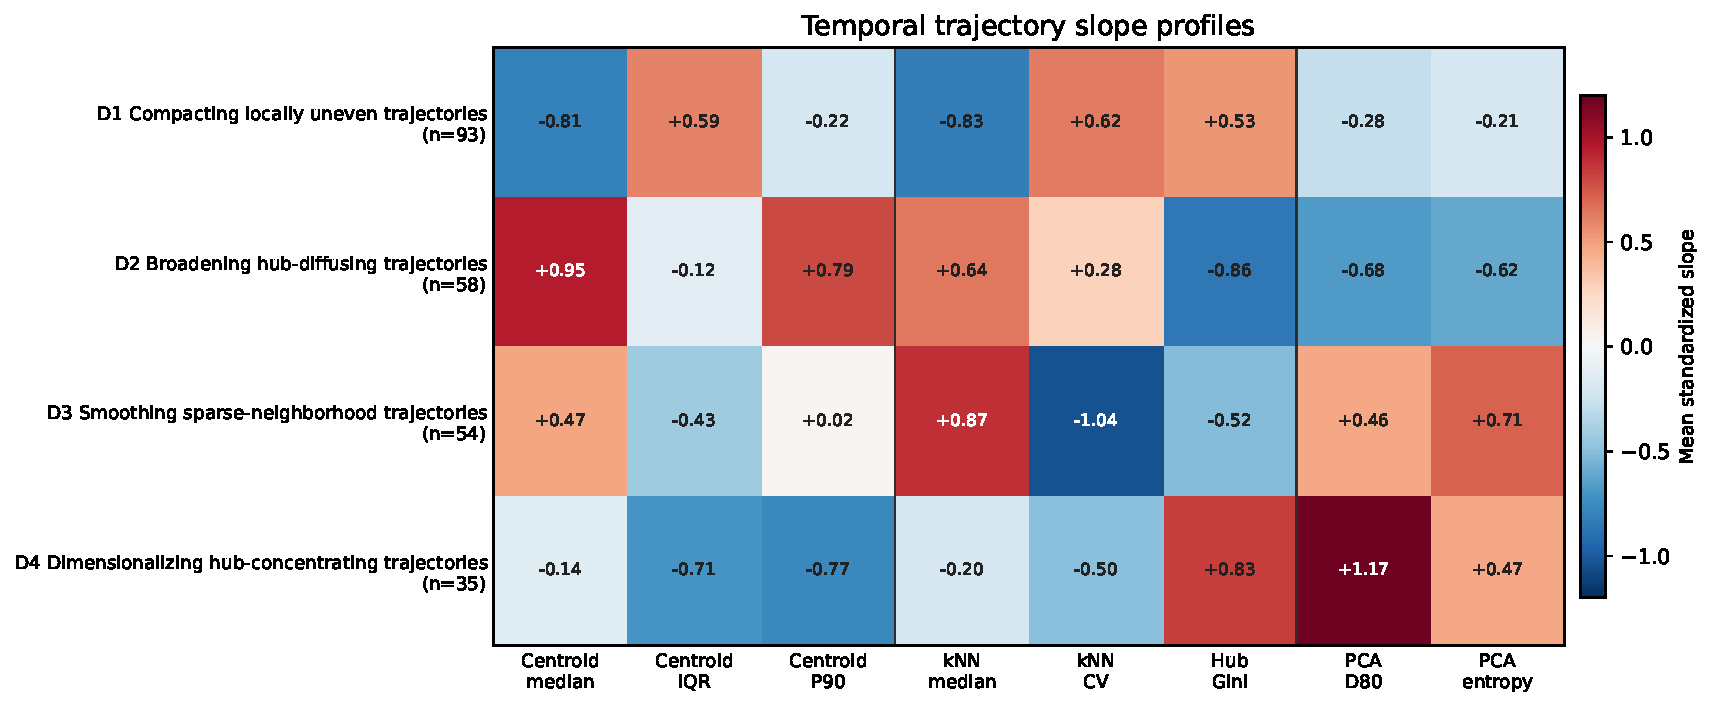
\includegraphics[width=\textwidth]{figures/fig_09_dynamic_typology_profile_heatmap.pdf}
\end{figure}

The four dynamic groups describe movement patterns. D1, with 93 subfields, contracts in centroid and kNN distance while local unevenness and hub concentration rise. D2, with 58 subfields, broadens while hubness and spectral complexity decline. D3, with 54 subfields, becomes sparser in local distance while local unevenness and hubness fall. D4, with 35 subfields, increases PCA dimensionality and hubness while outer spread and local variability fall. These labels are shorthand for slope profiles, not a new taxonomy.

The dynamic typology is useful because it gives names to repeated trajectory patterns. It should not be read as a new classification of science. The groups depend on the selected corpus, representation, metrics, windows, scaling, and clustering procedure. Their value is descriptive compression, not causal explanation. The main temporal result is that structural profiles move in heterogeneous but measurable ways, while centroid drift supplies a separate view of semantic displacement.
